\documentclass[12pt, openany]{report}
\usepackage[utf8]{inputenc}
\usepackage[T1]{fontenc}
\usepackage[a4paper,left=2cm,right=2cm,top=2cm,bottom=2cm]{geometry}
\usepackage[frenchb]{babel}
\usepackage{libertine}
\usepackage[pdftex]{graphicx}

\setlength{\parindent}{0cm}
\setlength{\parskip}{1ex plus 0.5ex minus 0.2ex}
\newcommand{\hsp}{\hspace{20pt}}
\newcommand{\HRule}{\rule{\linewidth}{0.5mm}}

\begin{document}

\begin{titlepage}
  \begin{sffamily}
  \begin{center}

    % Upper part of the page. The '~' is needed because \\
    % only works if a paragraph has started.
    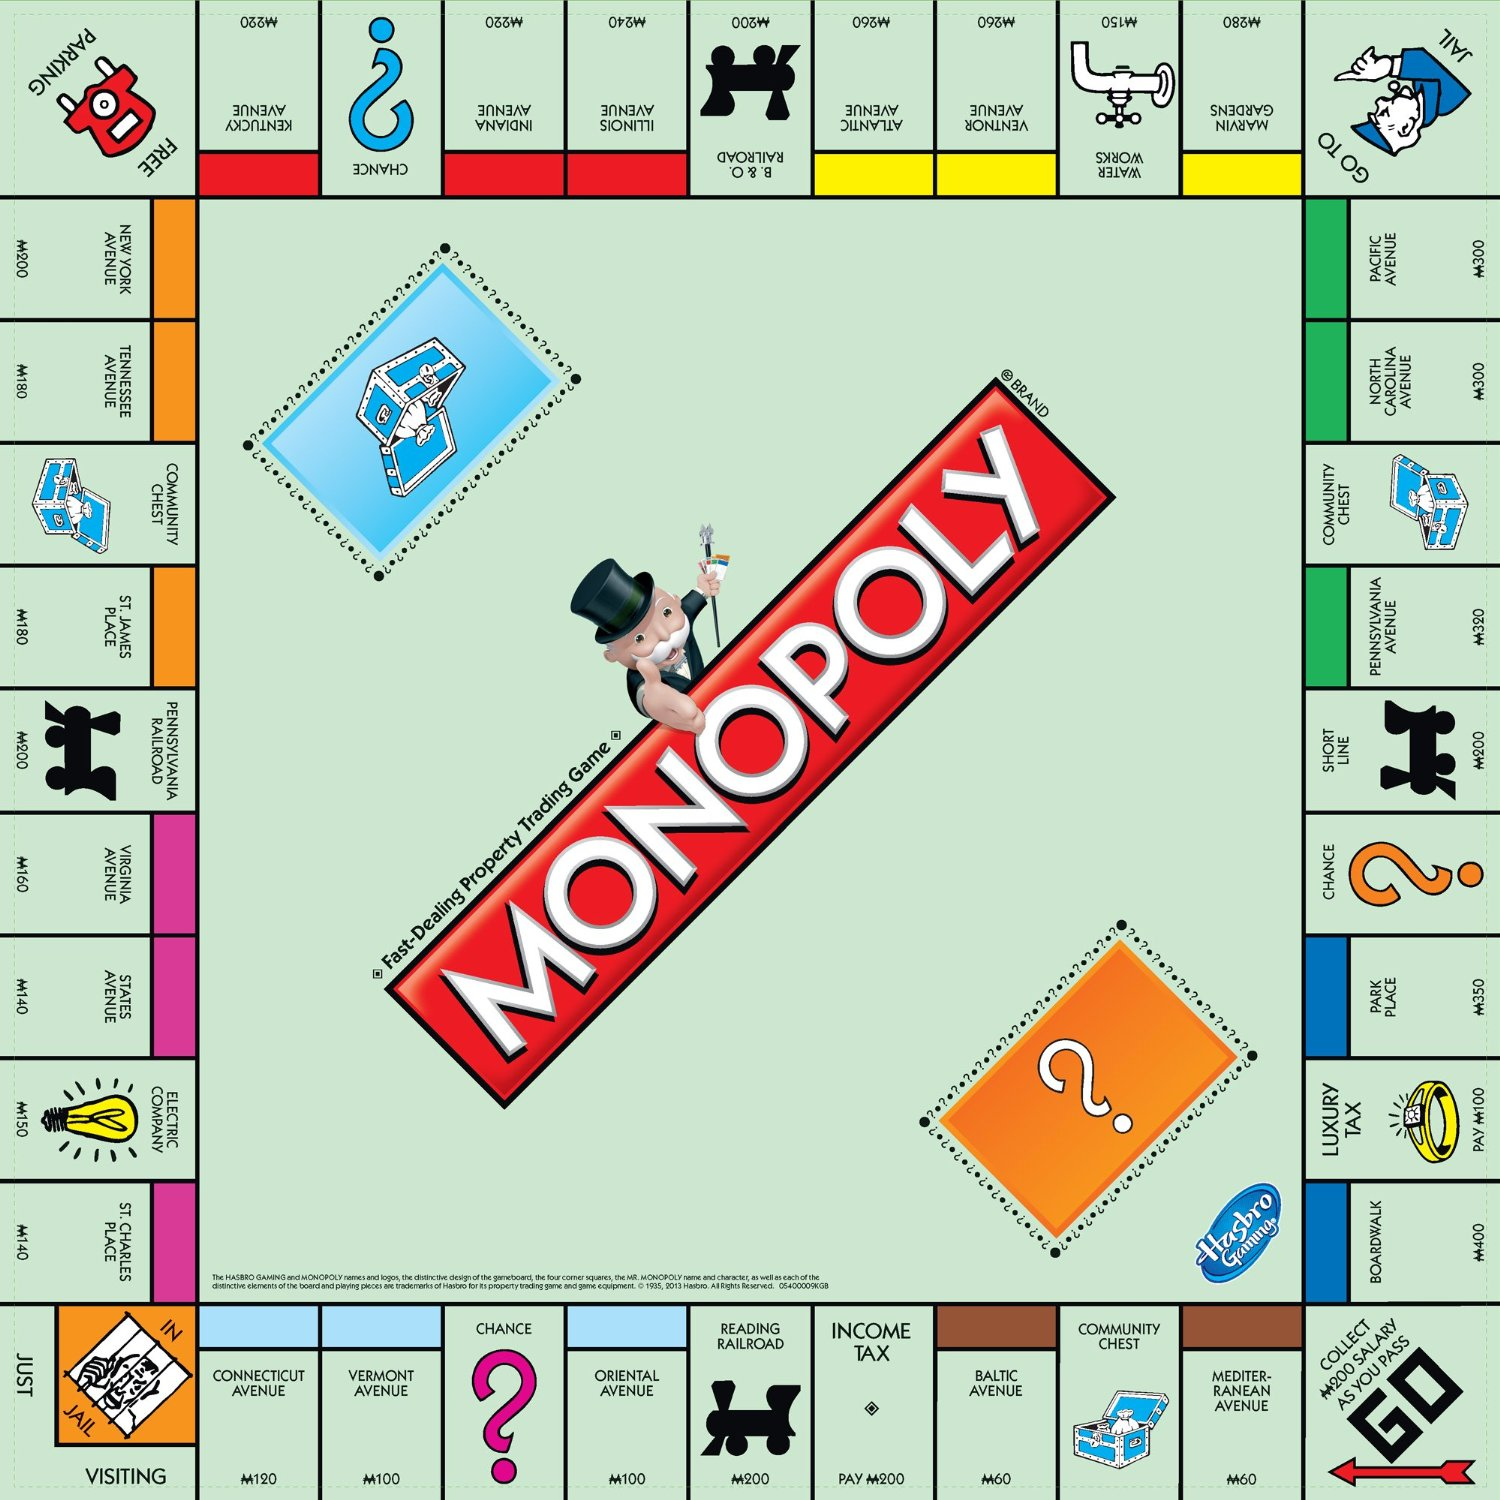
\includegraphics[scale=0.1]{monop.jpg}~\\[1.5cm]

    \textsc{\LARGE Faculté Jean Perrin, Lens}\\[2cm]

    \textsc{\Large Licence 3 Informatique}\\[1.5cm]

    % Title
    \HRule \\[0.4cm]
    { \huge \bfseries Rapport V.2 de projet, Monopoly\\[0.4cm] }

    \HRule \\[2cm]
    
\includegraphics[scale=0.3]{pions.jpg}
    \\[2cm]

    % Author and supervisor
    \begin{minipage}{0.4\textwidth}
      \begin{flushleft} \large
        Nicolas \textsc{Serf}\\
        Promo 2017\\
      \end{flushleft}
    \end{minipage}
    \begin{minipage}{0.4\textwidth}
      \begin{flushright} \large
        \emph{Professeur :} M. \textsc{Piette}\\
      \end{flushright}
    \end{minipage}

    \vfill

    % Bottom of the page
    {\large 22 Mars 2017}

  \end{center}
  \end{sffamily}
\end{titlepage}

\newpage
\section{Résumé}
Après le rendu du 21 mars de la premiére version du Monopoly, et le fait d'avoir réalisé que je n'avais pas assez travaillé ce projet, j'ai décidé de tout reprendre de 0 pour repartir sur de bonnes bases car le premier rendu avait une grande partie réalisé à la dernière minute. C'est ainsi que le fait de repartir de 0 m'a donné envie de réaliser une variante bien particuliére qui est la mise en réseau du Monopoly car ma première expérience du réseau avec la bataille navale m'a beaucoup plu. Cette variante va même plus loin comme je l'expliquerai dans ce rapport. C'est ainsi que pour ce projet, je suis réellement satisfait du travail que j'ai réalisé, en travaillant sans arrêt tout les jours, j'ai obtenu un résultat que j'attendais.
Ce rapport sera un peu plus particulier que le premier. En effet, dans le premier rapport, j'expliquais réellement tout les points de réflexion sur les différents choses qu'il allait falloir réaliser sur ce projet. Durant ce rapport, je m'axerais plus vers la technique du projet, en décrivant la partie réseau puis la partie client, et je décrirais le fonctionnement de l'application côté serveur et côté client. Ainsi, si vous voulez les informations sur les différentes tâches dans le jeu lui même a réaliser, référez vous au premier rapport.
\end{itemize}

\part{La partie réseau}
  \chapter{La réalisation de l'application serveur}
    \section{Réflexion sur la conception de mon serveur}
    Très bien commençons par expliquer comment j'ai pensé ma partie serveur. Durant la bataille navale, j'ai réalisé dans la même optique que ce projet, une partie étant réalisé avec 2 client qui communique avec un serveur. Durant le TP bataille navale, j'avais presque mis au point un serveur permettant de gérer plusieurs parties en même temps mais par manque de temps je n'avais pas pu le terminer.

C'est ainsi que j'ai voulu combler cette frustation rencontrée lors de la bataille navale en permettant à mon serveur de gérer plusieurs parties avec un nombre variable de joueur. J'ai même était plus loin en proposant un mini service de matchmaking.

En effet, c'était pour moi un défi de réaliser un mini service de matchmaking très simple (IE : lorsque assez de joueur recherche une partie, une partie est lancée avec ces derniers). Cette notion de matchmaking a neccesité la réalisation d'une connexion au serveur via un menu de connexion / d'inscription sur la partie client du projet.

Note : Pour la connexion / l'inscription et aussi les informations relative aux terrains, ces différents données sont enregistrées dans la base de données du serveur qui va pouvoir l'interroger à tout moment pour obtenir les informations dont il a besoin

Voici pour dégrossir les différents points qui m'ont orienté sur la réflexion pour la réalisation de mon serveur, je vais décrire dans la section en dessous l'explication de la réalisation de ce serveur.
    
    \section{La réalisation du serveur}
	\subsection{Le lancement du serveur}
	Comme expliqué, par la suite, pour un soucis de simplicité, toutes les configurations sont réalisés juste avant d'ouvrir le serveur, ici le port reste fixe car il n'a pas de sens à être changé. On peut choisir le nombre de joueur que l'on veut par partie, et ensuite s'en suit les différents configurations et variantes ou l'on peut choisir ce que l'on souhaite.
	
	\subsection{La connexion / l'inscription}
	Commençons par la première chose que voit un client lorsqu'il lance l'application et qui appel ainsi le serveur. Le client arrivé sur une page ou il a la possibilité de se connecter au serveur. Si celui-ci ne dispose pas de compte, il peut choisir de s'inscrire au serveur en premier lieu.

	Au niveau serveur, lorsqu'un client essaye de s'inscrire, une connexion en tant qu'inconnu est détecté, le serveur accepte cette connexion en sachant qu'il s'agit d'une demande d'inscription, il vérifie les différents informations d'inscription fournies par l'utilisateur. Si celles-ci sont valides (IE : pseudo pas déjà pris, mot de passe valide), le serveur répond positivement et l'inscription est réalisé dans la base de données du serveur. Le client est donc ensuite libre avec ces nouveaux identifiants de se connecter.

	Au niveau serveur, lorsqu'un client essaye de se connecter, une connexion en tant qu'inconnu est encore une fois détecté par le serveur, celui-ci vérifie les informations de connexion de l'utilisateur dans la base de données et dans le serveur (IE : identifiants correct et vérification que le client n'est pas déjà connecté), et répond en fonction. Si la réponse est positive, alors l'inconnu devient client avec comme identifiant son pseudo, et il est inséré dans la liste des clients du serveur avec un status lui étant propre (Connecté, occupé, absent, recherche de partie)

	Note : Toutes les communications et enregistrement de mot de passe des clients sont réalisés avec un hashage MD5 du mot de passe.

	\subsection{Le matchmaking}

	Une fois qu'un client est connecté sur le serveur, celui-ci est redirigé vers le lobby du serveur qui lui permet de consulter diverses choses qu'on verra dans la partie client. Cependant au niveau du serveur, un client peut choisir son statut de présence dans le serveur, celui-ci pouvant choisir entre les 4 choix suivants : 
	\begin{itemize}
	    \item En ligne
	    \item Absent
	    \item Occupé
	    \item En recherche de partie    
	\end{itemize}
Ces status sont visibles dans la fenetre du serveur mais surtout, ils sont enregistré pour chaque client. C'est le status 'en recherche de partie' qui nous intéresse puisque c'est celui-ci qui va permettre au matchmaking de savoir qu'un client peut participer à une partie. 

En effet, on trouve dans la partie serveur un Thread exécuté toutes les 1500 millisecondes qui permet de vérifier le nombre de client qui sont en recherche de partie, lorsque ceux-ci sont assez nombreux pour lancer une partie, une communication réseau est effectué pour lancer la partie avec les différents joueurs.

	\subsection{Le réseau en jeu}
	Petit chose qui n'a pas été précisé avant, lors du lancement du serveur, pour que celui-ci soit effectif, il faut configurer le serveur, ce qui signifie adapté comme on le souhaite les sommes de terrains et les différents variantes, cette partie a été réalisé dans le serveur pour une question de facilité puisque sinon, le matchmaking aurait du s'assurer que tout les joueurs disposer des mêmes options. Ainsi une instance de serveur va diriger les variantes de toutes les parties lancés avec celui-ci. Si l'on souhaite changer de variantes, il faut relancer le serveur.

La partie réseau est bien plus invisible en jeu. Une classe appelé GameEntity va gérer de elle même tout les communications qui sont réalisés entre les différents clients de la partie. On distingue 2 grandes phases pour l'entité qui gére le jeu. La premiére phase est une phase active, puisque l'entité construit les différents joueurs, analyse les différentes variantes et envoie toutes les informations aux différents joueurs en s'assurant que ceux-ci on bien reçu les instructions.

Une fois cette phase active réalisé, l'entité se trouve dans une forme passive ou elle ne fait qu'analyser les messages venant du controleur qui sont envoyés par les clients, et en fonction des messages, transmet à tout les joueurs ou seulement certains d'entres eux.

    \section{Le document de conception}
	Le diagramme de classe correspondant au serveur est le suivant : 

	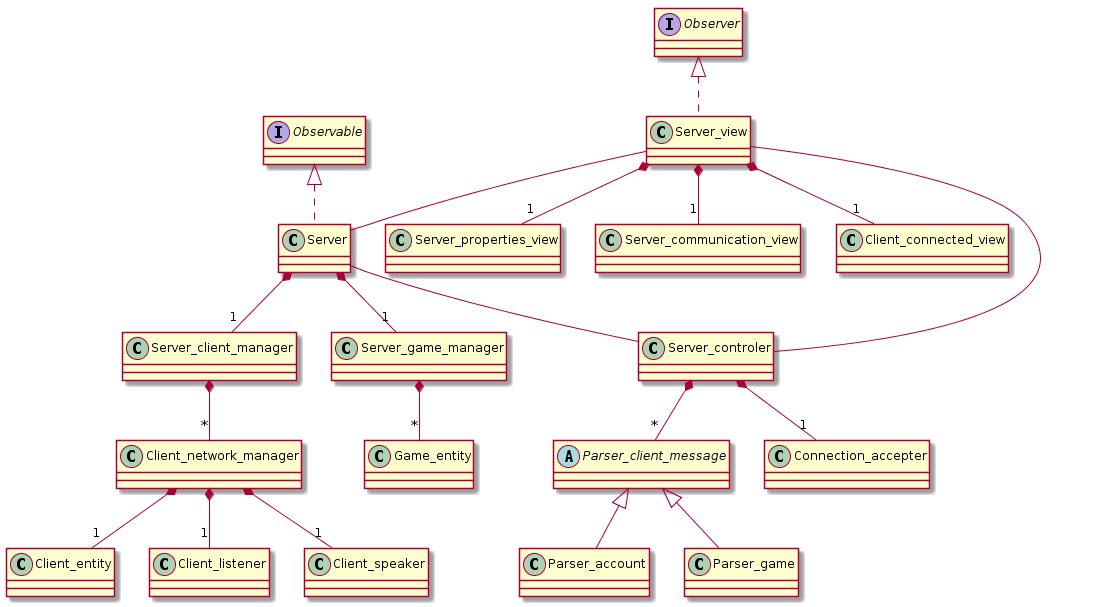
\includegraphics[scale=0.5]{diagram_server.png}

	Comment on peut le voir, la partie serveur respecte elle aussi le pattern MVC de manière adapté a ce dernier.

    \section{Conclusion sur le serveur}
	Voici qui clos l'explication bréve du serveur. On pourrait rentrer encore plus en détaille sur le fonctionnement du serveur mais ceci deviendrait inutilement compliqué pour comprendre le fonctionnement global du serveur. Voici résumé les différents grandes fonctionnalités du serveur :
    \begin{itemize}
	\item Gestion de compte avec connexion / inscription
	\item Gestion des utilisateurs avec status + gestion de déconnexion
	\item Gestion de matchmaking avec lancement lorsque assez de joueurs
	\item Gestion multi-partie pour gérer plusieurs parties en même temps avec nombre de joueur variable
	\item Gestion de partie avec deconnexion de joueur en partie et destruction des parties finies
	\item Un panel d'affichage serveur pour connaître les informations a tout moment
    \end{itemize}

    

\part{La partie client}
  \chapter{La réalisation de l'application client}
    \section{Réflexion sur la réalisation de mon client}
    Maintenant que nous avons vu la partie serveur, passons au client. Ayant fait mon premier rendu de monopoly pas en réseau et ou j'avais uniquement réalisé une petite partie du jeu, j'ai pu voir que ma conception n'était absolument pas propice à l'évolution et à un bon code objet. C'est pourquoi j'ai réalisé plusieurs petits diagrammes de classe sur papier avant de me lancer dans le développement. Je ne trouve pas beaucoup d'intêret à faire un diagramme de classe pour la partie interface de l'application ainsi j'ai de suite développé la partie menus sans m'appuier sur des diagrammes.

Comme nous allons le voir dans les sections qui suivent, j'ai réellement été étape par étape dans la réalisation de mon jeu, le réseau étant une contrainte supplémentaire ou je ne pouvais pas commencer le jeu sans avoir d'abord tout les joueurs prêt a débuter une partie, ainsi voici globalement la ligne que j'ai suivis pour le développement du client:

    \begin{enumerate}
        \item Réalisation de la partie réseau client
	\item Réalisation du menu de connexion / inscription + connexion au serveur
	\item Réalisation du menu de lobby avec le changement de status
	\item Réalisation dans le lobby des menus demandés (aide, crédits, difficultés, etc...)
        \item Réalisation de la création du plateau de jeu et initialisation
	\item Chargement des variantes
	\item Réalisation du jeu en lui même
	\item Test durant toutes les phases au dessus
    \end{enumerate} 

    \section {Réalisation du client}
	\subsection{Partie réseau du client}
	La partie réseau pour le client est ici bien moins compliqué que pour le réseau puisse qu'on a juste à gérer un seule communication sortante et un écouteur. Lorsque l'on se connecte, le serveur nous envoie l'autorisation de s'authentifier via notre pseudo. C'est ainsi que l'entité permettant de communiquer est créée. Cette entité dispose d'un écouteur qui a tout moment écoute les messages que pourrait lui envoyer le serveur.

On dispose d'un controleur de communication qui va s'occuper de gérer les différents ordres de communications, mais il ne présente pas un réel pattern MVC puisqu'on ne dispose pas de modéle et de vue a proprement parlé uniquement pour le réseau.

	\subsection{Menu de connexion et inscription}
	Le menu de connexion et d'inscription a été le premier code écrit hors réseau. Ce menu est essentiel puisqu'il permet de se connecter au serveur et de passer aux étapes suivantes (le lobby de l'application). Ici, si l'utilisateur n'est pas inscrit, il peut cliquer sur l'écriture rouge qui permet de switcher les différents sous panel pour s'inscrire.

A toute tentative de connexion / inscription, une communication réseau avec hashage MD5 pour le mot de passe est effectué avec le serveur pour vérifier les informations. Quand celle-ci sont valides, le client est connecté / inscrit. Une petite information supplémentaire, les pseudos ainsi que les mots de passe doivent rester un format alphanumérique stricte sans caractéres spéciaux ou espace.

Il n'y a pas grand chose à rajouter sur cette partie et l'application en elle-même sur cette partie parle assez bien d'elle même.
	
	\subsection{Menu de lobby}
	Le menu de lobby reste dans la même veine que le menu de connexion est parle assez bien de lui même. Dans le lobby, le client a le choix de choisir son statut courant entre les 4 valeurs et envoie cette valeur au serveur. Si le client est en recherche de partie, une petite animation se déclenche et le joueur doit attendre dans ce panel que le serveur trouve d'autre joueur pour jouer.

Dans ce même lobby, lorsque l'on ne se trouve pas en mode recherche de partie, on a accés aux autres menus demandés pour le projet, et on peut facilement naviguer entre ces menus pour trouver les informations.

	\subsection{Les différents menus}
	Il n'y a pas grand chose à expliquer sur les différents menus, ils présentent diverses informations me concernant, concernant le développement, les fonctionnalités, l'aide et les difficultés.

	\subsection{Création du plateau et initialisation}
	Voici une assez grosse partie qui m'a ici pris quelques jours. Dans ma première version, j'avais réalisé la création et l'affichage de mon plateau assez rapidement, seulement, comme je suis reparti de 0 avec de nouvelles structures de données et classes plus objet, j'ai du repensé tout le mécanisme d'affichage. Depuis, j'avais une variante supplémentaire ici qui est la prise en compte des différents variantes, et surtout l'initialisation du jeu par rapport aux variantes.

Cette étape c'est réalisé en 4 grosse étapes:
	\begin{itemize}
	    \item Le serveur envoie les différentes variantes à tout les clients qui prennent en compte ces variantes dans la configuration
	    \item Le serveur envoie les différentes valeures de terrain sous la forme JSON qui est lu via l'API GSON par le client pour construire les différents plateau
	    \item Le serveur envoi les différents joueurs avec leurs pseudos, leur position de jeu et leur position dans le plateau si une variante de position aléatoire est activé.
	    \item Le client dispose ici de toutes les informations du serveur, celui ci construire le plateau dans le modéle et dans le vue et une fois cette étape terminée, il notifie le serveur que tout est prêt.
	\end{itemize}

Cette étape se répéte biensur pour tout les joueurs qui se trouve dans la partie.
Une fois l'initialisation prête le jeu est prêt à se lancer mais cette partie m'a demandé beaucoup de temps car elle devait être totalement opérationnelle et sans bug pour pouvoir passer sur la réalisation du jeu en lui même puisque celui-ci a comme point de départ le plateau initialisé. J'ai de plus pas mal réfléchi a comment faire transister les informations avant de me rabattre sur le JSON.
Il faut savoir que pendant tout le temps ou l'application du client reçoit les informations du serveur et construit le plateau et l'interface qui demande un petit moment, une petite animation est présente à l'écran pour montrer que cette derniére n'a pas planté mais est bien en train de construire le plateau.

	\subsection{Réalisation du jeu}
	Passons probablement à la partie la plus longue de développement. Le jeu en lui même, le réseau n'aidant pas, il a fallut implémenter tout le jeu du monopoly avec ces régles de base et en intégrant les différents variantes qui sont présents dans le sujet.
Il serait long d'énumerer toutes les fonctionnalités puisque j'en oublierais certainement, et il serait long d'expliquer le code puisque celui-ci compte plus de 10000 lignes, mais voici briévement les fonctionnalités majeurs du jeu, je reviendrais sur certaines subtilités du monopoly et du réseau qui sont gérés par l'application pour souligner certains points.
	\begin{itemize}
	    \item Lancer le dés + gestion des dés + animation des dés
	    \item Gestion des pions déplacement + animation 
	    \item Achat / vente de propriété
	    \item Perte d'argent / Gain argent + animation perte d'argent
	    \item Ajout / retrait de maisons sur les propriétés avec affichage
	    \item Hypothéque / déhypothéque de maison avec affichage
	    \item Encheres avec affichage
	    \item Echange avec affichage
	    \item Fin de tour
	    \item Système de miniature pour permettre à tout le monde de connaitre les cartes des joueurs
	    \item Gestion des cartes chance et communauté avec affichage de la carte puis action
	    \item Zoom lors du passage de la souris sur les terrains du plateau pour connaitre les informations 
	    \item Gestion des différentes variantes
	    \item Gestion de la prison
	    \item Gestion du son
	    \item Gestion de la connexion / abandon des joueurs + affichage
	    \item Gestion de fin de partie avec vainqueur
	    \item Le tout étant gérer en réseau évidemment
	\end{itemize} 


Voici globablement les fonctionnalités même si il est possible que j'en ai oublié.
Il serait long de décrire chaque sous partie de fonctionnalité, mais globalement voici quelques points trompeurs ou j'ai du faire particuliérement attention, a cause du réseau ou non.


	\begin{itemize}
	    \item Des états bloquants (d'affichage et de modele) sont présents dés qu'il le faut
	    \item Il faut d'abord vendre des maison / propriété et hypothéquer si l'on a pas assez d'argent
	    \item La carte anniversaire ou tout le monde vous doit de l'argent réalise un état bloquant sur le joueur qui gagne l'argent en attendant que tout le monde ai payé
	    \item Perte d'argent / Gain argent + animation perte d'argent
	    \item Les enchéres sont gérés et s'actualise à chaque nouvelle enchére
	    \item Les échanges sont gérés via un panneau simple d'utilisation et des vérifications sont effectués en fonction des événements
	    \item Si un joueur quitte prématurement ou abandonne, des tests sont réalisés pour savoir si on doit passer au joueur suivant ou non
	\end{itemize}

    \section{Le son}
	Je n'ai pas grand chose à dire sur le son, celui-ci est fonctionnel et il permet de jouer 2 sons principaux, un son de théme durant toute la partie, et lorsqu'un joueur lance les dés, on trouve un son simulant un lancé de dés. 

	Nota bene : Je déconseille de mettre le son aprés l'avoir testé puisqu'avec plusieurs applications qui tourne en même temps, c'est tout bonnement horrible à l'oreille.

    \section{La messagerie instantannée}
	Monopoly en réseau oblige, il me paraissait essentiel d'intégrer un chat en ligne à ce dernier pour que les joueurs puissent par exemple communiqué par rapport à un échange. Ainsi, à gauche dans la partie interface, un chat est disponible ou l'on peut envoyer autant de message que l'on souhaite, ces derniers étant limité à 200 caractères chacun. La boite de message au dessus permet d'avoir les différents messages des joueurs via un JScrollPane pour les faire défiler

    \section{Les échanges}
	Bien que cette partie soit intégré au jeu de base, je vais briévement expliquer l'implémentation que j'en ai faite puisque le réseau vient encore une fois donner sa petite touche d'originalité.

Un joueur lorsqu'il souhaite échanger va appuyer sur le bouton "trade", a partir de ce menu, tout les joueurs disponibles dans la partie vont s'afficher et le joueur devra cliquer sur le nom de l'opposant avec qui il veut passer un échange. S'ouvre ensuite une fênetre d'échange ou le joueur trouvera à gauche ces biens, et à droite ceux proposés par l'adversaire. Pour selectionner un bien que l'on souhaite intégrer à l'échange, il suffit de cliquer sur le nom de la propriété, si on reclique une deuxiéme fois, cela enléve la propriété de l'échange. Il est aussi possible de donner de l'argent en mettant la somme dans le carré et en appuyant sur entrée ou sur l'écriture "Give". Lorsqu'un joueur a fini d'ajouter des élements, il peut cliquer sur valider qui grisera sa fênetre (ce qui sera aussi visible chez l'adversaire pour qu'il voit que celui ci est prêt a terminer l'échange). Si l'adversaire appuie sur valider, l'échange est effectué et tout les biens transitent entre les joueurs. Si un joueur effectue une modification alors que l'autre a valider, le status valide est enlevé et les deux joueurs doivent reconfirmer via le bouton "valider". Si un joueur quitte prématurément le jeu en pleins échange, alors l'échange est tout simplement annulé.

NOTE : Il faut noter que l'abandon est différent de la faillite. Une faillite n'est jamais décidé par le joueur, c'est l'application qui décide pour lui si il est déclaré en faillite. Lorsqu'un joueur abandonne, il est noté par un message différent et surtout, il ne gagne pas lors du mode suicide.

    \section{La faillite}
	Je vais aussi ici parler un peu de la faillite puisque celle-ci est un peu particuliére comme on joue via ordinateur. J'ai facilité les régles de faillite par rapport à un jeu plateau. Voici ainsi la ligne directrice.

Lorsqu'un joueur doit payer une somme, un petit panel s'affiche au milieu du plateau avec le bouton payer, si celui-ci est dans les capacités de payer (IE: son capital (et non son argent réel) le permet), alors le jeu reste bloqué ici jusqu'a ce que le joueur fasse en sorte de vendre pour pouvoir payer. Si la faillite est déclaré (IE: le capital n'est pas suffisant) alors le joueur voit un panneau de défaite apparaitre. Chez les autres joueurs, si le joueur est endetté envers un autre joueur, celui-ci gagne tout l'argent qu'il restait et les différents propriétés. Si l'endettement est envers la banque, alors toutes les propriétés sont de nouveaux disponibles à l'achat en tombant sur les cases.

    \section{La bonne foi}
Un dernier point avant a mes variantes personnelles est la bonne foi qui doit être demandé à chaque joueur. En effet, le jeu s'appuyant sur des états bloquants au moment des tours des joueurs, les joueurs doivent faire preuve de bonne foi et finir le tour lorsqu'ils en ont la possibilité, etc...

    \section{Mes variantes personnelles}
        Ma premiére variante concerne la vente de maison. En effet, il y a maintenant dans mon plateau de jeu à côté des cartes la possibilité d'appuyer sur un bouton 'vente' qui permet de vendre immédiatement sans être obligé qu'une personne veuille faire un accord, à la banque notre propriété à 80\% de son prix d'achat. Cette variante est intéréssante puisqu'on peut très bien vouloir se faire plus d'argent que l'hypothéque tout en vendant sa propriété immédiatement qui sera donc de nouveau libre à l'achat.
\\
	Ma deuxiéme variante elle est configurable dans les autres variante du jeu, elle permet de choisir si l'on souhaite activer ou non le fait d'aller en prison aprés la réalisation de 3 doubles / triples. C'est un variante assez simple comparé à la premiére mais elle trouve tout de même son sens ludique et amusant, car combien de fois on espére ne pas réaliser 3 fois un double, ici cela permet de rendre le jeu un peu plus dynamique avec moins de temps de pause pour les joueurs chanceux !

    \section{La déconnexion prématurée}
Les déconnexions des deux cotés clients et serveur sont gérées (il est tout de même demandé de ne pas killer le processus brutalement pour un soucis évident d'intégrité de la partie). En effet, lorsqu'un joueur ne clique pas sur "Surrend" mais sur la croix pour quitter l'application, cette derniére s'occupe d'avertir le serveur et la partie ou il se trouve pour permettre aux autres joueurs de continuer la partie en donnant la main si c'était son tour par exemple.

Du côté serveur, on trouve le même comportement, si celui-ci est stoppé ou est fermé via la croix, alors les clients sont avertis de la fermeture du serveur et une fenêtre apparait pour leur signaler que le serveur est down.

    \section{Le document de conception}
	Le diagramme de classe correspondant au jeu de la partie client est le suivant : 

	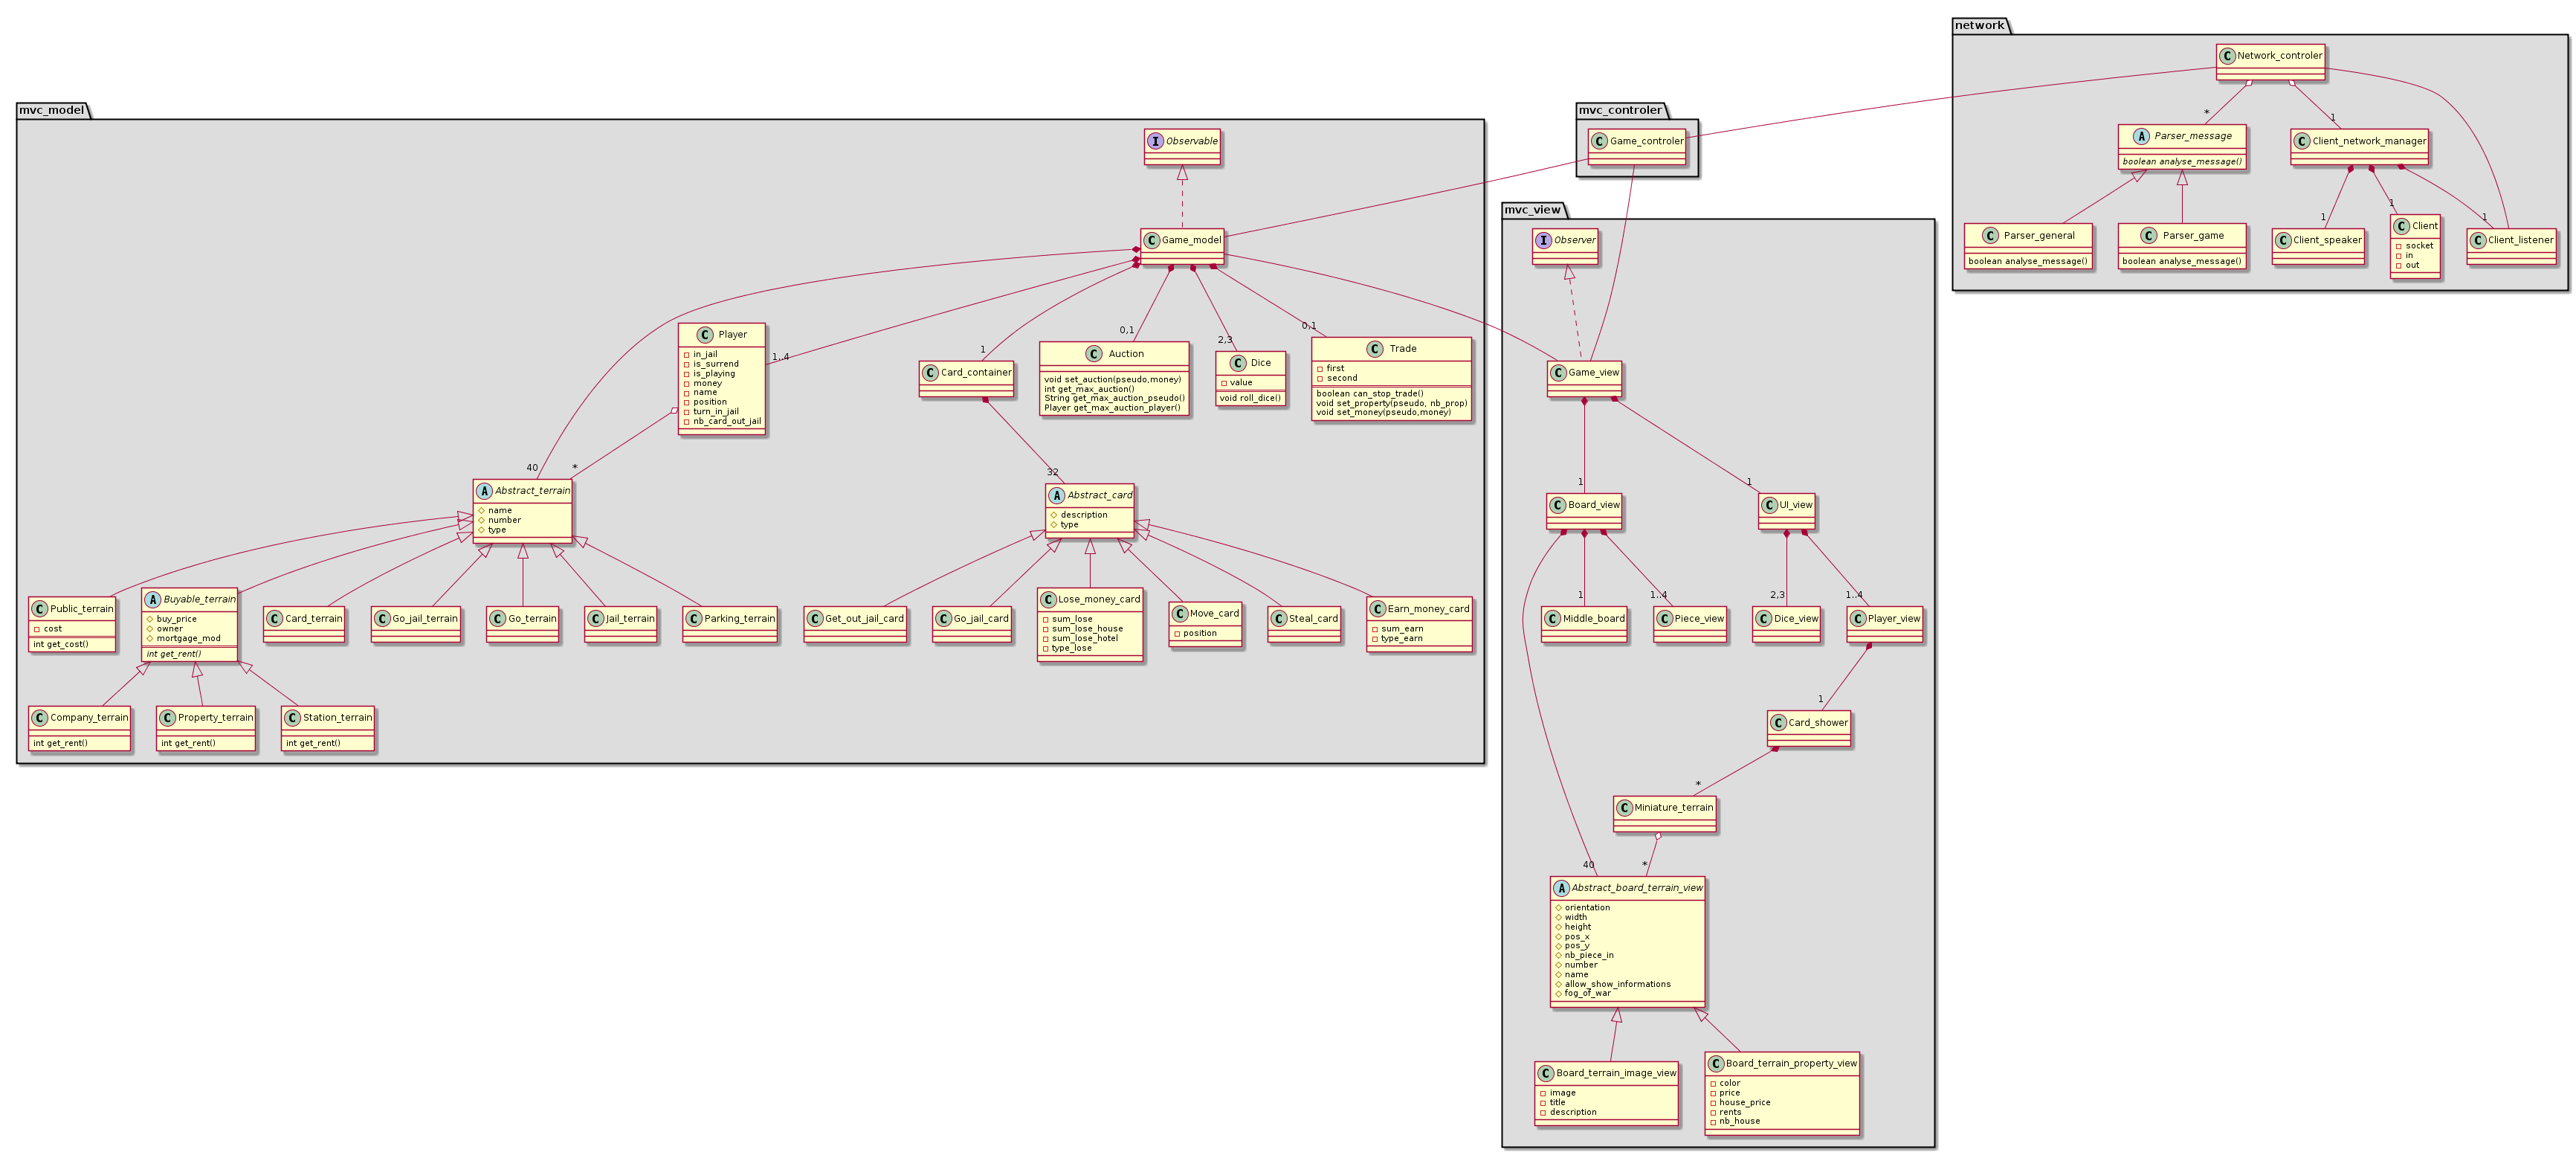
\includegraphics[scale=0.15]{diagram_game.png}

	On ne voit rien sur ce plan car le diagramme est assez large et surtout a cause des namespaces qui donne une disposition horizontale au diagramme, on peut trouver dans le dossier rapport/diagrammes/diagram\_game.png un diagramme ou l'on voit bien mieux le diagramme. Comment on peut le voir, la partie jeu du client respecte le pattern MVC de manière adapté a ce dernier.
	
    \section{Conclusion sur la partie client}
Passons à la conclusion sur la partie client. Je suis assez satisfaite de celle-ci dans le modéle, l'optimisation et la communication réseau. Le seul gros bémol reste pour moi les graphismes qui restent tout de même très simple et ne proposant rien de transcendant. J'ai toutefois préféré misé sur un jeu assez complet et un peu moins beau graphiquement. Car je ne suis rendu compte que j'avais perdu beaucoup de temps lors de la réalisation des menus pour proposer des choses agréables à l'oeil et je n'aurais pas eu le temps de finir ce que je voulais en faisant de même sur le jeu.

\part{Conclusion sur le projet}
  \chapter{Difficulté, ce qu'il reste à faire, ma conclusion générale}
    \section{Mes difficultés sur le projet}
    Plusieurs points que j'ai décide de réaliser sur ce projet m'ont causé des soucis, dont le principal qui est biensur la mise en réseau et tout ce que cela implique par rapport à un jeu qui ne se joue que sur une seule application.
Il serait long d'énumérer toutes les difficultés et quand bien même, il y en a certaines dont je ne me souviens plus mais voici les grands points qui me viennent à l'esprit:
      \begin{itemize}
        \item Le réseau de manière générale et les communications que cela implique
        \item La construction du plateau et la réflexion pour obtenir quelque chose de flexible
        \item La gestion des différentes variantes et ne rien oublier
        \item La mise en place du multi-partie sur le serveur
	\item Les tests de manière générale nécessitant de relancer tous les clients
	\item La gestion de fin de partie avec beaucoup d'état différent en fonction de l'abandon, faillite et du mode suicide
      \end{itemize}

    \section{Ce qui n'est pas implémenté}
      \begin{itemize}
        \item La variante : carte mixte
        \item La variante : choix du nombre de dés à chaque tour
	\item La variante : choix du plateau
	\item Une IA
	\item La sauvegarde
	\item Le changement de commandes 
      \end{itemize}


Je vais expliquer pour chaque point pourquoi il n'a pas été réalisé :
      \begin{itemize}
        \item Carte mixte : Mon architecture réseau me permettait trés difficilement de réaliser cette variante sans réaliser quelque chose de trés sale et qui m'aurait pris beaucoup de temps
        \item Le nombre de dés à chaque tour : En cours, la variante été presque fini mais l'architecture de la vue des dés m'a bloqué pour terminer cela, donc on peut choisir dans le milieu le nombre de dés, mais cela reste factice !
	\item Choix du plateau : Manque de temps, en effet cette variante demande énormément de temps car il faut adapter les cartes chances / communautés, le plateau, le nom des maisons et les images
	\item Une IA : Mon architecture me permettait encore une fois difficilement de réaliser l'IA même si cela aurait pu être possible, je trouvais l'idée de l'IA pour le monopoly de plus moins intérésante et c'est pourquoi j'ai préféré réaliser le réseau
	\item La sauvegarde : Presque impossible à réaliser à cause de la couche réseau + matchmaking, en effet chaque joueur est matché en partie avec un inconnu dés que celui-ci est connecté et en recherche de partie, il aurait fallu enregistrer chaque joueur et que le matchmaking reconnaisse chaqu'un d'entre eux et qu'ils disent tous si ils veulent charger une partie ou non. Cela représentait beaucoup de travail pour quelque chose qui dans la logique n'arrive que trés peu.
	\item Le changement de commandes : Manque de temps
      \end{itemize}

    \section{Ce que j'aurais aimé finir}
      \begin{itemize}
        \item Réaliser un design plus soigné pour le plateau de jeu
        \item J'aurais aimé faire une restructuration partielle d'une grosse partie du code.
        \item Réaliser les explications plus détaillées sur l'aide
      \end{itemize}

    \section{Bug}
Je n'ai pas vraiment trouvé de bug au niveau gameplay ou application, si des régles ne semblent pas correcte c'est simplement un oubli a par les 3 variantes citées au dessus ! Il subsiste à ma connaissance un seul bug assez génant qui n'arrive que trés trés rarement et qui n'est pas arrivé depuis un moment est lors du chargement des plateaux, il arrive que ceux ci se figent car une configuration n'a apparement pas pu être transféré, il faut donc relancer les différents clients.

    \section{Conclusion générale}
J'aurais beaucoup de choses à dire en tant que conclusion générale, mais je vais essayer de me reduire au minimum. Assez réticent au premier abord, le projet ne m'attirais pas du tout (j'ai beucoup de mal à être attiré par les projets de jeux que je ne concois pas moi même dans les régles) mais il s'est révélé que le projet était en fin de compte très intéressant à programmer et il reprennait de plus tout les concepts vu en cours, durant j'ai projet j'ai ainsi utilisé : Le réseau, les Thread, le XML, les bases de données, JSON qui sont des notions vues en cours. J'ai beaucoup appris sur la mise en place d'un communication client / serveur et si le projet était à refaire, il est certain que je referai encore autrement car j'ai appris beaucoup de mes erreurs pendant ce projet, et certaines erreurs ou 'mauvaises conceptions' que j'ai du retravaillé pour les incorporés au projet par manque de temps que j'aurais changé si j'avais eu plus de temps.

Ainsi, je ressors grandis sur ce projet sur deux grands points, la conception et la réseau et je suis finalement assez satisfait du travail réalisé.
\end{document}


